\documentclass[12pt]{article}
\usepackage{graphicx}
\usepackage[none]{hyphenat}
\usepackage{graphicx}
\usepackage{listings}
\usepackage[english]{babel}
\usepackage{graphicx}
\usepackage{caption} 
\usepackage{booktabs}
\usepackage{array}
\usepackage{amssymb} % for \because
\usepackage{amsmath}   % for having text in math mode
\usepackage{extarrows} % for Row operations arrows
\usepackage{listings}
\lstset{
  frame=single,
  breaklines=true
}
\usepackage{hyperref}
  
%Following 2 lines were added to remove the blank page at the beginning
\usepackage{atbegshi}% http://ctan.org/pkg/atbegshi
\AtBeginDocument{\AtBeginShipoutNext{\AtBeginShipoutDiscard}}
\usepackage{gensymb}


%New macro definitions
\newcommand{\mydet}[1]{\ensuremath{\begin{vmatrix}#1\end{vmatrix}}}
\providecommand{\brak}[1]{\ensuremath{\left(#1\right)}}
\providecommand{\sbrak}[1]{\ensuremath{{}\left[#1\right]}}
\providecommand{\norm}[1]{\left\lVert#1\right\rVert}
\providecommand{\abs}[1]{\left\vert#1\right\vert}
\newcommand{\solution}{\noindent \textbf{Solution: }}
\newcommand{\myvec}[1]{\ensuremath{\begin{pmatrix}#1\end{pmatrix}}}
\let\vec\mathbf


\begin{document}

\begin{center}
\title{\textbf{Convex Optimization}}
\date{\vspace{-5ex}} %Not to print date automatically
\maketitle
\end{center}
\setcounter{page}{1}

\section{11$^{th}$ Maths - Chapter 10}
This is Problem-3.1 from Exercise 10.3 
\begin{enumerate}
\item Reduce $x-\sqrt{3}y+8=0$ into normal form. Find its perpendicular distance from the origin and angle between perpendicular and the positive x-axis. 

\solution 
The given equation can be written as
\begin{align}
	\label{eq:Eq1}
	\myvec{1 \\ -\sqrt{3}}^\top\vec{x}+8 &= 0 \\
	\implies \vec{n} = \myvec{1 \\ -\sqrt{3}} \\
	\implies \vec{m} = \myvec{1 \\ \frac{1}{\sqrt{3}}}
\end{align}
Equation \eqref{eq:Eq1} can be represented in parametric form as
\begin{align}
	\label{eq:Eq2}
	\vec{x} = \vec{A}+\lambda\vec{m}
\end{align}
Here, $\vec{A}$ is a point on the given line. 

Let $\vec{O}$ be the point from where we have to find the perpendicular distance. The perpendicular distance will be the minimum distance from $\vec{O}$ to the line. Let $\vec{P}$ be the foot of the perpendicular. This problem can be formulated as an optimization problem as follow:
\begin{align}
	\label{eq:Eq3}
	&  \min_{\vec{x}} \norm{\vec{x}-\vec{O}}^2\\
	& \text{s.t.} \quad \vec{n}^T\vec{x} = c 
\end{align}
\begin{enumerate}
\item Using parametric equation:

Substituting \eqref{eq:Eq2} in \eqref{eq:Eq3}
\begin{align}
	& \implies \min_{\lambda} \norm{ \vec{A}+\lambda\vec{m} -\vec{O}}^2\\
	& \implies \min_{\lambda} \norm{ \lambda\vec{m} +\brak{\vec{A}-\vec{O}}}^2\\
	&\implies f\brak{\lambda} = \sbrak{\lambda\vec{m}+ \brak{\vec{A}-\vec{O}}}^\top \sbrak{\lambda\vec{m}+ \brak{\vec{A}-\vec{O}}} \\  
	&= \sbrak{\lambda\vec{m^\top}+ \brak{\vec{A}-\vec{O}}^\top} \sbrak{\lambda\vec{m}+ \brak{\vec{A}-\vec{O}}} \\  
	&= \lambda^2\norm{\vec{m}}^2+ \lambda\brak{\vec{A}-\vec{O}}^\top\vec{m}+ \lambda\vec{m}^\top\brak{\vec{A}-\vec{O}}+ \norm{\vec{A}-\vec{O}}^2 \\  
	\label{eq:Eq4}
	&= \lambda^2\norm{\vec{m}}^2+ 2\lambda\brak{\vec{A}-\vec{O}}^\top\vec{m}+  \norm{\vec{A}-\vec{O}}^2  
\end{align}
$\because$ the coefficient of $\lambda^2> 0$, equation \eqref{eq:Eq4} is a convex function.
\begin{align}
	f^\prime\brak{\lambda} &= 2\lambda\norm{\vec{m}}^2+ 2\brak{\vec{A}-\vec{O}}^\top\vec{m}
\end{align}	
\begin{align}
	f^{\prime\prime}\brak{\lambda} &= 2\norm{\vec{m}}^2 \\ 
	\because f^{\prime\prime}\brak{\lambda} > 0, f^\prime\brak{\lambda_{min}} &= 0, \text{ for } \lambda_{min}
\end{align}
\begin{align}
	& f^\prime\brak{\lambda_{min}} =  2\lambda_{min}\norm{\vec{m}}^2 + 2\brak{\vec{A}-\vec{O}}^\top\vec{m}  = 0 \\
	\label{eq:EqMin}
	\lambda_{min} &= -\frac{\brak{\vec{A}-\vec{O}}^\top\vec{m}}{\norm{\vec{m}}^2} 
\end{align}
We choose  
\begin{align}
	\vec{A} &= \myvec{-8 \\ 0}\\
	\vec{O} &= \myvec{ 0 \\ 0}
\end{align}
Substituting the values of $\vec{A}$, $\vec{O}$ and $\vec{m}$ in equation \eqref{eq:EqMin}
\begin{align}
	\lambda_{min} &= -\frac{\brak{\myvec{-8 \\ 0 }-\myvec{0 \\ 0}}^\top\myvec{1 \\ \frac{1}{\sqrt{3}}}}{\norm{\myvec{1 \\ \frac{1}{\sqrt{3}}}}^2}\\ 
	&= \frac{\myvec{8 & 0 }\myvec{1 \\ \frac{1}{\sqrt{3}}}}{\frac{4}{3}}\\ 
	&= 6
\end{align}
Substituring this value in equation \eqref{eq:Eq2}
\begin{align}
	\vec{x}_{min} &= \vec{P} = \myvec{-8 \\ 0}+6\myvec{1 \\ \frac{1}{\sqrt{3}}}  \\
	&= \myvec{-8 \\ 0}+\myvec{6 \\ \frac{6}{\sqrt{3}}} \\
	&= \myvec{-2 \\ 2\sqrt{3}} \\
	OP &= \norm{\vec{P}-\vec{O}}^2 \\ 
	&= \norm{\myvec{-2 \\ 2\sqrt{3}}-\myvec{0 \\ 0}} \\
	&= \sqrt{2^2 + 12} = \sqrt{16} = 4
\end{align}
\item Solving using cvxpy, with 
\begin{align}
	&\vec{n} = \myvec{1 \\ -\sqrt{3}} \\
	&\vec{O} = \myvec{0 \\ 0} \\
	&c = -8 \\
	\label{eq:minval}
	&  \min_{\vec{x}} \norm{\vec{x}-\vec{O}}^2 = 4, 
	 \vec{x}_{min} = \myvec{-2  \\ 3.46 } 
\end{align}
\end{enumerate}
The angle $\theta$ made by this perpendicular with x-axis is given by
\begin{align}
         \theta &= \tan^{-1}\brak{\frac{2\sqrt{3}}{-2}} \\
	 &= \tan^{-1}\brak{-\sqrt{3}} \\
	 &= 120\degree
\end{align}
The normal form of equation for straight line is given by
\begin{align}
	\myvec{\cos120\degree \\ \sin120\degree}^\top\vec{x} &= 4 
\end{align}
The relevant figures are shown in \ref{fig:Fig1} and \ref{fig:Fig2}
\begin{figure}[!h]
	\begin{center}
		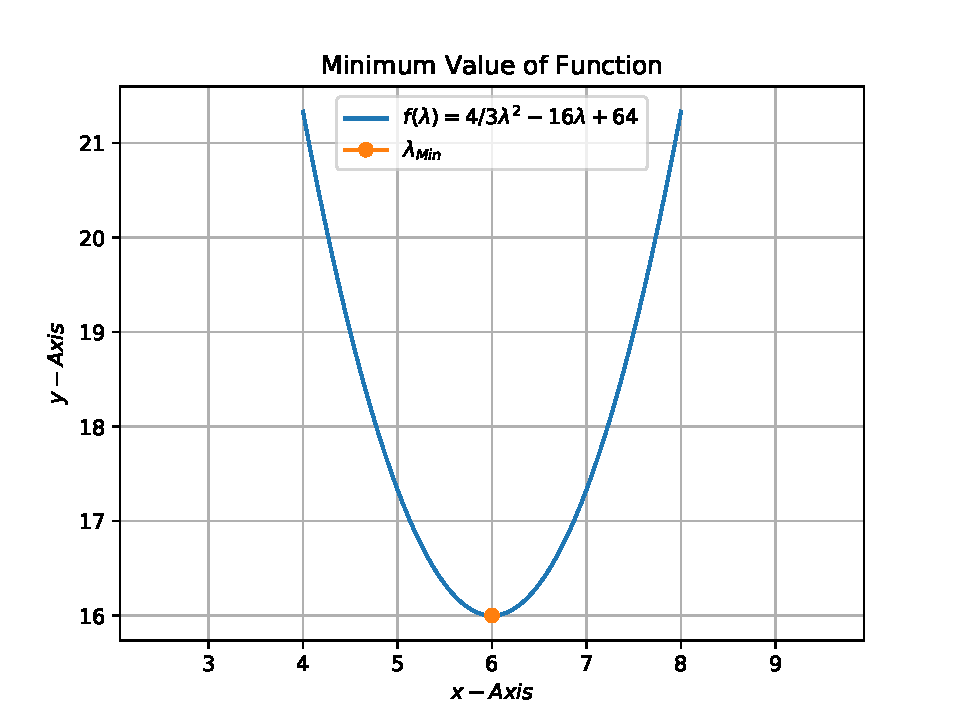
\includegraphics[width=\columnwidth]{figs/problem3.1a.pdf}
	\end{center}
\caption{}
\label{fig:Fig1}
\end{figure}
\begin{figure}[!h]
	\begin{center}
		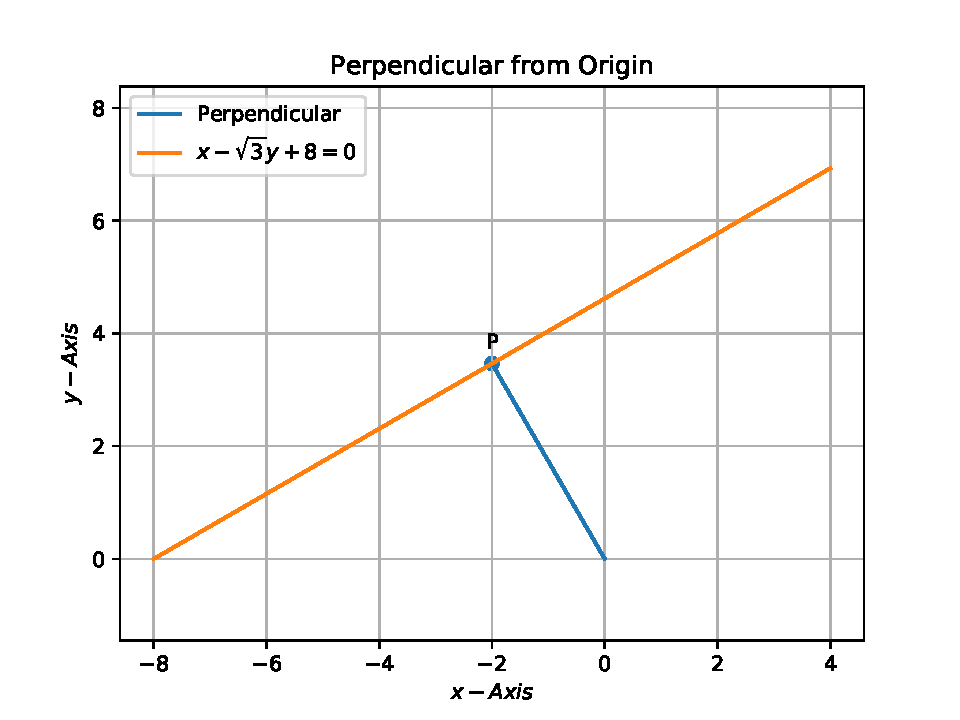
\includegraphics[width=\columnwidth]{figs/problem3.1b.pdf}
	\end{center}
\caption{}
\label{fig:Fig2}
\end{figure}
\end{enumerate}
\end{document}
